\documentclass[journal]{IEEEtran}

\usepackage[T1]{fontenc}
\usepackage{lmodern}
\usepackage{amsmath,amssymb}
\usepackage{booktabs}
\usepackage{graphicx}
\usepackage{tabularx}
\usepackage[table]{xcolor}
\usepackage{tikz}
\usetikzlibrary{arrows.meta,positioning,fit,calc}
\usepackage{microtype}
\usepackage[hidelinks]{hyperref}
\usepackage{url}

\newcommand{\systemname}{TPG-Fact}
\newcommand{\datasetname}{US-TPMFC}
\newcolumntype{Y}{>{\raggedright\arraybackslash}X}
\definecolor{tpgblue}{HTML}{1F5A94}
\definecolor{tpgteal}{HTML}{167D75}
\definecolor{tpgviolet}{HTML}{6A4C93}
\definecolor{tpgorange}{HTML}{B65C20}
\definecolor{tpggray}{HTML}{4B5563}

\title{Temporal and Evidence-Source Provenance-Aware Multimodal Misinformation Detection with Calibrated Abstention}

\author{Sabbir Hossain%
\thanks{S. Hossain is with the Department of Computer Science, American International University-Bangladesh, Dhaka, Bangladesh (e-mail: \href{mailto:26-94030-1@student.aiub.edu}{26-94030-1@student.aiub.edu}).}}

\begin{document}
\maketitle

\begin{abstract}
An authentic photograph can still spread misinformation when it is paired with the wrong event, place, or time. Multimodal fact-checkers often retrieve web evidence to identify such false context, but retrieval introduces three risks: the model may use documents published after the decision cutoff, mistake syndicated copies for independent corroboration, or issue a confident verdict when the available evidence is inadequate. This study proposes \systemname{}, a temporal and evidence-source provenance-aware framework for classifying image--text claims as supported, refuted, or insufficient evidence. The framework combines lexical, dense, and visual retrieval; removes post-cutoff items; organizes claims, documents, images, publishers, hyperlinks, and publication order in a heterogeneous graph; and aggregates evidence by source-dependency cluster. A hierarchical classifier estimates evidence sufficiency before veracity, while temperature scaling and a validation-selected threshold enable selective abstention. The study also specifies \datasetname{}, a temporally partitioned benchmark design built from United States ClaimReview cases and open web archives. Training spans 2020--2023, validation uses 2024, and testing uses 2025--2026, with events, near-duplicate claims, and reused images kept within a single partition. The evaluation compares matched multimodal retrieval baselines and tests temporal leakage, duplicate-source sensitivity, calibration, and selective risk. Together, this protocol tests whether time-valid, independently sourced evidence improves future-event decisions and reduces overconfidence.
\end{abstract}

\begin{IEEEkeywords}
multimodal misinformation, automated fact-checking, evidence provenance, temporal retrieval, selective prediction, calibrated abstention
\end{IEEEkeywords}

\section{Introduction}

Digital misinformation often reuses genuine media outside its original context. A photograph from one event may be paired with a claim about another place, date, or incident. This form of out-of-context misinformation is difficult to detect from pixels alone because the image may contain no manipulation artifacts. Pairwise image and text compatibility can reveal a mismatch, but it cannot establish what the image originally depicted or whether the accompanying claim is true. NewsCLIPpings and VERITE illustrate the need to evaluate false context separately from synthetic or visibly edited media \cite{luo2021newsclippings,papadopoulos2024verite}. A fact-checking system therefore needs external evidence that links the claim and image to real events.

Retrieval supplies that context, but the validity of a decision depends on when the evidence appeared and where it originated. For a claim assessed at cutoff time $\tau$, a later correction, official report, or fact-check page contains information that was unavailable at the time of the decision. Allowing such documents into evaluation leaks future information and can inflate measured performance. Search results can also give a false impression of corroboration. Syndicated articles, reposts, and quotation chains may produce many documents that trace back to one report. Document-level aggregation can therefore overweight a single underlying source.

Evidence availability is different from model confidence. The task uses three verdict labels. \emph{Supported} means that time-valid evidence corroborates the claim, \emph{refuted} means that it contradicts the claim, and \emph{insufficient evidence} means that the available material cannot settle the claim. Selective abstention is a separate model decision: the system may defer any prediction when its calibrated confidence is too low. This separation permits independent measurement of evidential sufficiency and decision reliability.

Recent systems address parts of this setting. MOCHEG connects multimodal retrieval with verification \cite{yao2023mocheg}; RED-DOT reranks web evidence by relevance \cite{papadopoulos2025reddot}; and COVE recovers an image's original context before assessing its caption \cite{tonglet2025cove}. KAMP incorporates background knowledge graphs \cite{zhang2025kamp}, while RAGAR and MultiReflect use retrieval-augmented multimodal reasoning \cite{khaliq2024ragar,kangur2025multireflect}. The present study places four concerns in the same decision pipeline: temporal eligibility, source dependence, evidence sufficiency, and calibrated deferral.

This study asks whether time-valid evidence from independent source clusters improves future-event misinformation detection and reduces overconfident decisions relative to ordinary multimodal RAG. Each case is an English claim about a United States event, accompanied by an image and a decision cutoff. \systemname{} filters evidence by publication time, groups dependent sources, represents provenance in a heterogeneous graph, and estimates evidence sufficiency before veracity. Its output includes a verdict, calibrated class probabilities, the selected evidence identifiers, source-cluster identifiers, and the cutoff used for the decision.

The study makes three contributions:
\begin{itemize}
    \item a construction and audit protocol for \datasetname{}, a temporally partitioned benchmark derived from professional fact-check metadata and open web archives, with events, near-duplicate claims, and reused images isolated by split;
    \item a temporal-provenance framework that combines multimodal retrieval, cutoff filtering, source-dependency clustering, graph-based evidence aggregation, hierarchical sufficiency and veracity prediction, and calibrated abstention; and
    \item a controlled evaluation protocol covering future-event generalization, temporal leakage, duplicated-source sensitivity, retrieval quality, calibration, selective risk, and event-level uncertainty.
\end{itemize}


\section{Related Work}

\subsection{Multimodal Misinformation Detection}

NewsCLIPpings introduced a large benchmark of authentic news images paired with deliberately mismatched captions \cite{luo2021newsclippings}. VERITE later addressed unimodal bias and topic imbalance in real-world evaluation \cite{papadopoulos2024verite}. KAMP uses single-modality, cross-modal, and knowledge-content objectives during multimodal pretraining \cite{zhang2025kamp}. Other work uses synthetic examples to improve transfer to real misinformation cases \cite{zeng2024synthetic}. Event-Radar represents visual manipulation, textual emotion, and event-level inconsistency in an event graph \cite{ma2024eventradar}. These methods provide the main no-retrieval and event-aware baselines in this study.

\subsection{Evidence-Grounded Fact-Checking}

MOCHEG treats multimodal fact-checking as a sequence of evidence retrieval, claim verification, and explanation generation \cite{yao2023mocheg}. MetaSumPerceiver summarizes evidence drawn from several multimodal documents \cite{chen2024metasum}. RED-DOT accounts for irrelevant web evidence through relevance-aware reranking \cite{papadopoulos2025reddot}. RAGAR and MultiReflect combine multimodal language models with retrieval and iterative reasoning \cite{khaliq2024ragar,kangur2025multireflect}, and SNIFFER retrieves external material for out-of-context detection \cite{qi2024sniffer}. The proposed method builds on this retrieval setting while enforcing publication-time cutoffs and aggregating evidence by source dependency.

\subsection{Image Context, Time, and Evidence Dependence}

The 5Pils system recovers an image's original context from web evidence \cite{tonglet2024image}, and COVE predicts that context before assessing a caption \cite{tonglet2025cove}. Chronological distribution shift can reduce the accuracy of multimodal misinformation models \cite{stepanova2023temporal}. ChronoFact handles complex temporal claims with structured timeline reasoning \cite{barik2025chronofact}. Source information also affects how RAG-based fact verification resolves conflicting evidence \cite{ge2025conflicting}. This study represents publication time and source dependence in the same evidence graph.


\section{Task and Benchmark Construction}

\subsection{Task Definition}

Each instance contains claim text $x_t$, an image $x_v$, a decision cutoff $\tau$, and an evidence collection $E_{\leq\tau}$. The output is $y \in \{\text{supported},\text{refuted},\text{insufficient}\}$. Documents published after $\tau$ are unavailable to the model. The event is the independent unit for data splitting and uncertainty analysis.

\subsection{Candidate Acquisition}

Corpus construction starts with English ClaimReview records about United States events from 2020--2026. GDELT provides discovery metadata, and Common Crawl provides archived page observations. The corpus retains cases with an identifiable claim time, a recoverable image or archive, an unambiguous professional rating, and enough timestamp information to enforce the cutoff. The retrieval pool excludes fact-check domains and documents that contain the final verdict.

\subsection{Label Policy}

Only explicit site ratings are normalized. True or correct maps to supported. False, fake, or miscaptioned maps to refuted. Unproven, unsubstantiated, or no evidence maps to insufficient evidence. Mixed, partially true, satire, opinion, and ambiguous ratings are excluded. The labels come from professional fact-checkers; automatically extracted evidence links are treated as silver evidence.

\subsection{Temporal Partitioning and Release}

Training covers 2020--2023, validation uses 2024, and final testing uses 2025--2026. Events, near-duplicate claims, and images with matching perceptual hashes remain in one partition. The release package contains URLs, cryptographic and perceptual hashes, timestamps, normalized labels, graph annotations, retrieval queries, and split manifests. It does not redistribute copyrighted articles or images.

Figure~\ref{fig:temporal-protocol} shows the order of operations. Group identities are fixed before the year-based allocation. Training data are used to fit model parameters and preprocessing; validation data are reserved for model selection, calibration, and abstention thresholds; the final period is not used for any of those choices.

\begin{figure}[t]
\centering
\resizebox{\columnwidth}{!}{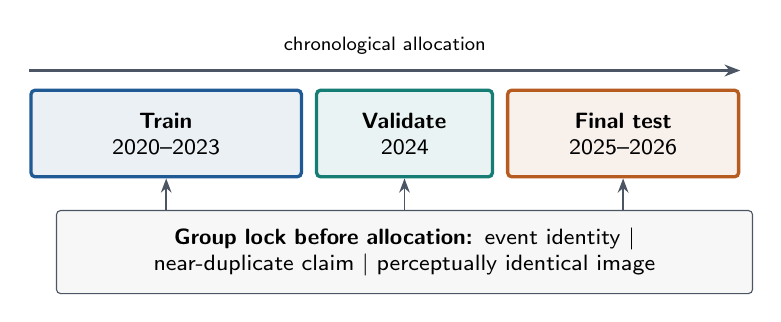
\begin{tikzpicture}[
  font=\sffamily\footnotesize,
  phase/.style={draw, very thick, rounded corners=1.5pt, minimum height=11mm, align=center},
  guard/.style={draw=tpggray, rounded corners=1.5pt, fill=black!3, align=center, inner sep=2.2mm}
]
  \node[phase, draw=tpgblue, fill=tpgblue!9, text width=32mm] (train) {
    \textbf{Train}\\2020--2023
  };
  \node[phase, draw=tpgteal, fill=tpgteal!9, text width=20mm, right=1.5mm of train] (val) {
    \textbf{Validate}\\2024
  };
  \node[phase, draw=tpgorange, fill=tpgorange!9, text width=27mm, right=1.5mm of val] (test) {
    \textbf{Final test}\\2025--2026
  };

  \draw[-{Stealth[length=2mm]}, very thick, draw=tpggray]
    ([yshift=8mm]train.west) -- ([yshift=8mm]test.east)
    node[midway, above=0.7mm, font=\sffamily\scriptsize] {chronological allocation};

  \node[guard, text width=84mm, below=4mm of val] (lock) {
    \textbf{Group lock before allocation:}
    event identity $\mid$ near-duplicate claim $\mid$ perceptually identical image
  };
  \draw[-{Stealth[length=1.8mm]}, semithick, draw=tpggray] (lock.north -| train) -- (train.south);
  \draw[-{Stealth[length=1.8mm]}, semithick, draw=tpggray] (lock.north -| val) -- (val.south);
  \draw[-{Stealth[length=1.8mm]}, semithick, draw=tpggray] (lock.north -| test) -- (test.south);

\end{tikzpicture}
}
\caption{Primary temporal split and leakage controls. A locked event, near-duplicate claim, or reused image cannot cross partitions.}
\label{fig:temporal-protocol}
\end{figure}

This study treats \datasetname{} as a benchmark only if the filtered corpus contains at least 2,000 cases, 300 cases per label, 50 test events, and two independent evidence clusters for at least 70\% of retained claims. If the collection misses any threshold, it is used as a temporal and provenance stress test instead.


\section{Temporal-Provenance Method}

\subsection{Framework Overview}

Figure~\ref{fig:pipeline} follows one claim from retrieval to a traceable decision. The cutoff controls which evidence may enter the graph, while source clustering controls how that evidence is counted. These constraints act before the hierarchical classifier and therefore cannot be repaired by calibration after an invalid or duplicated evidence set has already been aggregated.

For claim $c$ and evidence pool $E$, the retained set is
\begin{equation}
E_{\leq\tau}^{(k)}=\operatorname{TopK}_{k}\{r(c,e):e\in E,\ t(e)\leq\tau\},
\label{eq:time-filter}
\end{equation}
where $r(c,e)$ is the fused retrieval score, $t(e)$ is the best available publication timestamp, and $k=20$. The provenance stage maps this set to dependency clusters $C(E_{\leq\tau}^{(k)})$ before graph encoding.

\begin{figure*}[t]
\centering
\resizebox{\textwidth}{!}{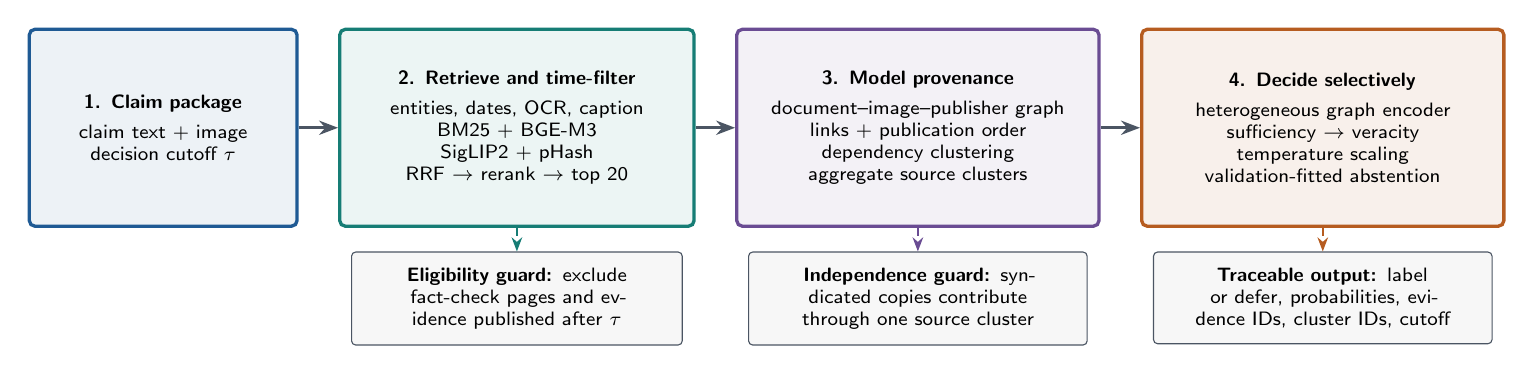
\begin{tikzpicture}[
  font=\sffamily\scriptsize,
  stage/.style={
    draw,
    very thick,
    rounded corners=2pt,
    align=center,
    minimum height=25mm,
    inner sep=3.5mm
  },
  flow/.style={-{Stealth[length=2.4mm,width=1.8mm]}, very thick, draw=tpggray},
  note/.style={
    draw=tpggray,
    rounded corners=1.5pt,
    fill=black!3,
    align=center,
    inner sep=2mm,
    font=\sffamily\scriptsize
  }
]
  \node[stage, draw=tpgblue, fill=tpgblue!8, text width=27mm] (claim) {
    \textbf{1. Claim package}\\[1mm]
    claim text + image\\
    decision cutoff $\tau$
  };

  \node[stage, draw=tpgteal, fill=tpgteal!8, text width=38mm, right=5mm of claim] (retrieve) {
    \textbf{2. Retrieve and time-filter}\\[1mm]
    entities, dates, OCR, caption\\
    BM25 + BGE-M3\\
    SigLIP2 + pHash\\
    RRF $\rightarrow$ rerank $\rightarrow$ top 20
  };

  \node[stage, draw=tpgviolet, fill=tpgviolet!8, text width=39mm, right=5mm of retrieve] (graph) {
    \textbf{3. Model provenance}\\[1mm]
    document--image--publisher graph\\
    links + publication order\\
    dependency clustering\\
    aggregate source clusters
  };

  \node[stage, draw=tpgorange, fill=tpgorange!9, text width=39mm, right=5mm of graph] (decision) {
    \textbf{4. Decide selectively}\\[1mm]
    heterogeneous graph encoder\\
    sufficiency $\rightarrow$ veracity\\
    temperature scaling\\
    validation-fitted abstention
  };

  \draw[flow] (claim) -- (retrieve);
  \draw[flow] (retrieve) -- (graph);
  \draw[flow] (graph) -- (decision);

  \node[note, below=3mm of retrieve, text width=38mm] (cutoff) {
    \textbf{Eligibility guard:} exclude fact-check pages and evidence published after $\tau$
  };
  \node[note, below=3mm of graph, text width=39mm] (independence) {
    \textbf{Independence guard:} syndicated copies contribute through one source cluster
  };
  \node[note, below=3mm of decision, text width=39mm] (output) {
    \textbf{Traceable output:} label or defer, probabilities, evidence IDs, cluster IDs, cutoff
  };

  \draw[-{Stealth[length=1.8mm]}, semithick, dashed, draw=tpgteal] (retrieve) -- (cutoff);
  \draw[-{Stealth[length=1.8mm]}, semithick, dashed, draw=tpgviolet] (graph) -- (independence);
  \draw[-{Stealth[length=1.8mm]}, semithick, dashed, draw=tpgorange] (decision) -- (output);
\end{tikzpicture}
}
\caption{End-to-end \systemname{} pipeline. The temporal guard removes unavailable evidence, provenance clustering prevents copies from being treated as independent corroboration, and the final record preserves the evidence trail. Selective deferral is applied to the calibrated three-class prediction and is not a fourth task label.}
\label{fig:pipeline}
\end{figure*}

\subsection{Time-Constrained Multimodal Retrieval}

For each claim, retrieval begins with named entities, temporal expressions, OCR text, and an image caption. BM25 and BGE-M3 retrieve text candidates, while SigLIP2 embeddings and perceptual hashes retrieve images. Reciprocal-rank fusion merges the lexical, dense, and visual rankings. A reranker processes the top 100 candidates, and the system keeps the 20 highest-ranked items that satisfy the publication-time cutoff.

\subsection{Evidence-Source Provenance Graph}

The graph contains nodes for claims, images, documents, publishers, entities, and events. Typed edges record retrieval relevance, image containment, near-duplicate content, hyperlinks, publisher membership, entity or event mentions, and temporal order. Document clusters are estimated from exact hashes, MinHash-style lexical similarity, semantic similarity, perceptual image distance, hyperlinks, and publication order. The earliest observed document is an origin candidate because the available records may not reveal the original author.

Let $C(E)$ denote the partition of evidence documents into dependency clusters. The model first aggregates documents within a cluster and then combines information across clusters. As a result, repeated copies of one report do not receive the same weight as several independent sources.

\subsection{Hierarchical Decision and Abstention}

A heterogeneous graph transformer encodes the temporal-provenance graph for the claim. The sufficiency head estimates $p(s=1\mid x,E_{\leq\tau})$. Sufficient evidence passes to a veracity head that predicts supported or refuted; the remaining cases receive the insufficient-evidence label. Temperature scaling is fitted to validation predictions, and an abstention threshold is selected on the same split to target 80\% answer coverage. Each prediction records class probabilities, evidence identifiers, source clusters, and the enforced cutoff.


\section{Experimental Protocol}

\subsection{Baselines}

The controlled comparison includes majority prediction, text-only classification, image--text fusion without retrieval, and an open multimodal language model under zero- and few-shot prompting. Retrieval baselines cover vanilla multimodal RAG, time-filtered RAG without provenance, provenance-aware RAG without time filtering, and RED-DOT where its implementation is compatible with the protocol. Every method uses the same splits, candidate corpus, evaluation code, and 20-trial validation budget.

\subsection{Metrics and Statistical Analysis}

The primary metric is macro-F1 on the 2025--2026 event-disjoint test set. Secondary metrics are per-class F1, balanced accuracy, macro one-versus-rest AUROC, Brier score, negative log-likelihood, expected calibration error, area under the risk--coverage curve, risk at 80\% coverage, Recall@10, nDCG@10, latency, GPU memory, and retrieved-document count. Final configurations are evaluated with five seeds. Differences use 10,000 paired event-level bootstrap replicates, with Holm correction across the primary comparison family.

\subsection{Ablation and Stress Tests}

The ablations remove temporal filtering, dependency clustering, temporal edge features, graph aggregation, text evidence, visual evidence, the sufficiency gate, and evidence-dropout training one at a time. The stress tests add syndicated copies and post-cutoff documents that reveal the verdict. They also remove the earliest observed source, introduce conflicts between dependent and independent evidence, swap captions, and reuse historical images.

\subsection{Selection and Falsification Rules}

Hyperparameters and the abstention threshold are selected using validation data only. Evidence-source provenance must improve either future-event performance or resistance to duplicate injection to support a performance claim. Calibrated abstention must reduce selective risk at matched coverage. Gains that depend on post-cutoff documents count as leakage.

Table~\ref{tab:evaluation-matrix} links each intended claim to a controlled comparison and an explicit rejection condition. This keeps the interpretation tied to tests that can fail rather than to a favorable result chosen after evaluation.

\begin{table*}[t]
\caption{Claim-to-test matrix for the main empirical questions. Each comparison uses the same event-disjoint temporal split and evidence corpus unless the named stress test changes the evidence.}
\label{tab:evaluation-matrix}
\centering
\footnotesize
\setlength{\tabcolsep}{4pt}
\renewcommand{\arraystretch}{1.12}
\begin{tabularx}{\textwidth}{>{\raggedright\arraybackslash}p{0.19\textwidth}YYY}
\toprule
\textbf{Question} & \textbf{Controlled comparison} & \textbf{Primary readout} & \textbf{Evidence that would reject the claim} \\
\midrule
Does decision-time filtering help? & Full model vs. vanilla RAG and provenance-only RAG & Test macro-F1 and leakage sensitivity & No advantage outside settings containing post-cutoff evidence \\
\rowcolor{black!4}
Does provenance prevent copy inflation? & Cluster aggregation vs. document aggregation with 1, 5, and 10 injected copies & Confidence shift, Brier score, selective risk, macro-F1 & Similar degradation under duplicate injection \\
Does sufficiency-first prediction help? & Hierarchical decision vs. flat three-class classifier & Insufficient-evidence F1, macro-F1, AURC & No sufficiency gain or higher risk at matched coverage \\
\rowcolor{black!4}
Does calibration support useful deferral? & Temperature-scaled vs. uncalibrated confidence at equal coverage & Risk at 80\% coverage and AURC & Selective risk does not decrease at matched coverage \\
\bottomrule
\end{tabularx}
\end{table*}



\section{Evaluation Questions}

The first analysis tests whether excluding post-cutoff documents changes retrieval quality and future-event classification. The full method is compared with vanilla multimodal RAG and with provenance-aware RAG that does not enforce a time cutoff. Event-level paired bootstrap intervals quantify the differences.

The second analysis measures how source dependence affects a verdict. It compares cluster-level aggregation with document-level aggregation before and after injecting one, five, and ten syndicated copies of the same source. Changes in macro-F1, confidence, Brier score, and selective risk show whether repeated evidence is being counted as independent corroboration.

The third analysis examines the sufficiency gate and calibrated abstention. A flat three-class classifier and an uncalibrated confidence threshold provide matched controls. The comparison uses insufficient-evidence F1, area under the risk--coverage curve, and risk at 80\% coverage.


\section{Discussion, Ethics, and Limitations}

The main methodological risk is mistaking repeated web coverage for independent corroboration. Dependency clusters can only use observable content, links, domains, and timestamps. They cannot prove that two publishers worked independently or identify the original author with certainty. Archive timestamps show when a page was observed, which may be later than its first publication.

The corpus inherits professional fact-check labels and the editorial policies behind them. Restricting the mapping to explicit ratings reduces ambiguity, but it can also create selection bias and class imbalance. The focus on United States events and English sources limits geographic and linguistic generalization. Common Crawl and GDELT do not cover the whole web, and blocked or deleted pages may differ systematically from the pages that remain available.

The release will not redistribute copyrighted articles or images without permission. It will contain URLs, hashes, derived metadata, split manifests, and collection code. The system is meant for research and assisted review, not autonomous censorship or content removal. An insufficient-evidence prediction calls for further investigation; it does not mean that the claim is false.


\section{Conclusion}

This study examines whether a multimodal fact-checker benefits from knowing when evidence appeared and when several documents came from the same source. \systemname{} enforces a decision-time cutoff, groups dependent evidence before aggregation, checks whether the retrieved material is sufficient, and abstains when confidence is too low. The evaluation separates ordinary future-event performance from gains caused by temporal leakage and repeated documents. Its ablations also test whether the graph, source clusters, and sufficiency gate earn their place in the model. The final claims depend on controlled comparisons; a large stack of web documents does not count as corroboration on its own.



\bibliographystyle{IEEEtran}
\bibliography{references}

\end{document}

